\section{Additional figures}

\begin{figure}[h]
\centering
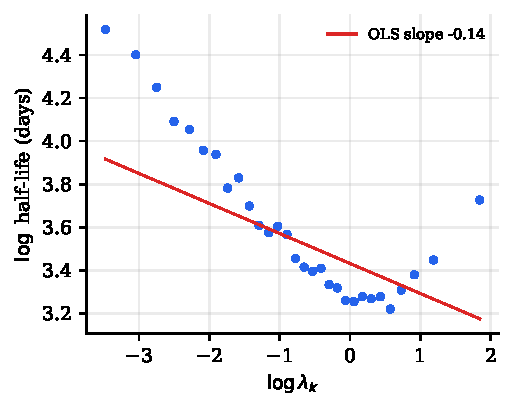
\includegraphics[width=0.48\textwidth]{ou_halflife}
\caption{In-window AR(1) half-life of the cumulative mode price against
$\log\lambda_k$, all modes and episodes (medians in 30 eigenvalue bins).
The OU model \eqref{eq:prediction} predicts slope $+1$; the fitted slope
is \OUSlope. \OUNoRev\% of mode-windows show no detectable reversion
($b\ge1$) and are excluded from the fit.}
\label{fig:ou}
\end{figure}

\begin{figure}[h]
\centering
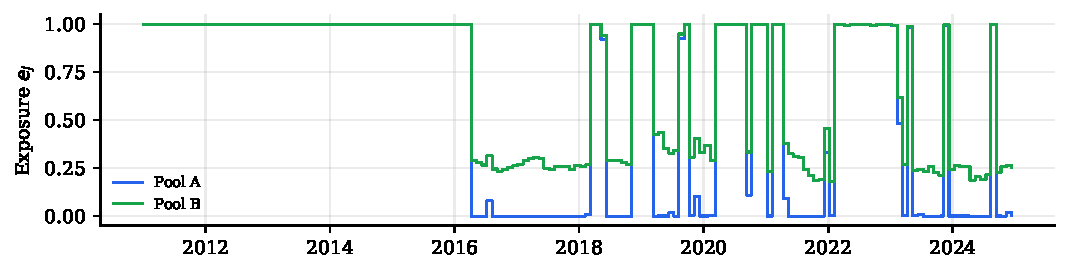
\includegraphics[width=\textwidth]{exposure}
\caption{Walk-forward regime-overlay exposure $e_j$ for the ML strategies.
Average exposure is \MeanExpA{} (Pool~A) and \MeanExpB{} (Pool~B).}
\label{fig:exposure}
\end{figure}


\section{Implementation details}

\paragraph{HMM estimation.} Baum--Welch uses the scaled forward--backward
recursions of \citet{rabiner1989}. It is initialized by splitting the
sample into volatility terciles (halves, for two states), with a
transition matrix of 0.98 on the diagonal, and runs to a log-likelihood
tolerance of $10^{-6}$. Variances are floored at $10^{-4}$ in
standardized units. The first fit uses data from 2010 to 2011 and
produces probabilities from January 2012.

\paragraph{Leakage checks.} The test suite (\texttt{tests/}) perturbs
future data and verifies that nothing computed for the past changes. It
covers the signal, every episode feature, the HMM filter, the
walk-forward HMM refits, and the walk-forward classifier, which is
checked to be invariant to future labels. It also checks that a
single-mode portfolio reproduces the sign of that mode's standalone
PnL, and that the HMM recovers known states on synthetic data.

\paragraph{Reproduction.} \texttt{python scripts/run\_study.py} downloads
the data (cached), runs every stage, and writes all figures and tables
in this paper together with \texttt{output/results.json}.
\texttt{python scripts/make\_macros.py} then regenerates every number
quoted in the text. A full run takes about ten minutes on a laptop.
